\chapter{Conclusions and Discussion}
\label{conclutions}

The work presented in this thesis has made it possible to design and begin producing the next-generation polarized $^3$He targets for use at Jefferson Laboratory. These next-generation targets are being developed and produced in two steps, which are referred to internally at JLab as the Stage-I and Stage-II designs. The Stage-I targets contain a volume of 3 STP liters of $^3$He, the same quantity that was contained in the cell Antoinette, the results from which were described in Chapter 4. The Stage-II targets, while similar in geometry, are larger and will contain 6 STP liters of $^3$He. At the time of this writing, the first Stage-I target cell has already been produced and is undergoing bench tests. When using only half the design laser power, the target has already achieved a polarization of 65\%, higher than what is needed for actual running (although we note that this is without the depolarizing effects of an electron beam). These early tests are quite encouraging when extrapolated to the full laser power that
will be used. Also, the conceptual design of the Stage-II target cells has been 
completed, and was evaluated in a review, conducted in March of 2016, of the polarized $^3$He target that is being built for the Hall A Super Bigbite Spectrometer (SBS) experiment to measure $G_E^n$ (E12-09-016), the electric form factor of the neutron. The design for the SBS $G_E^n$ target is shown in Fig~\ref{Next_Gen_Design}.

\begin{figure}[t!]
	\centering
	\resizebox{0.91\textwidth}{!}{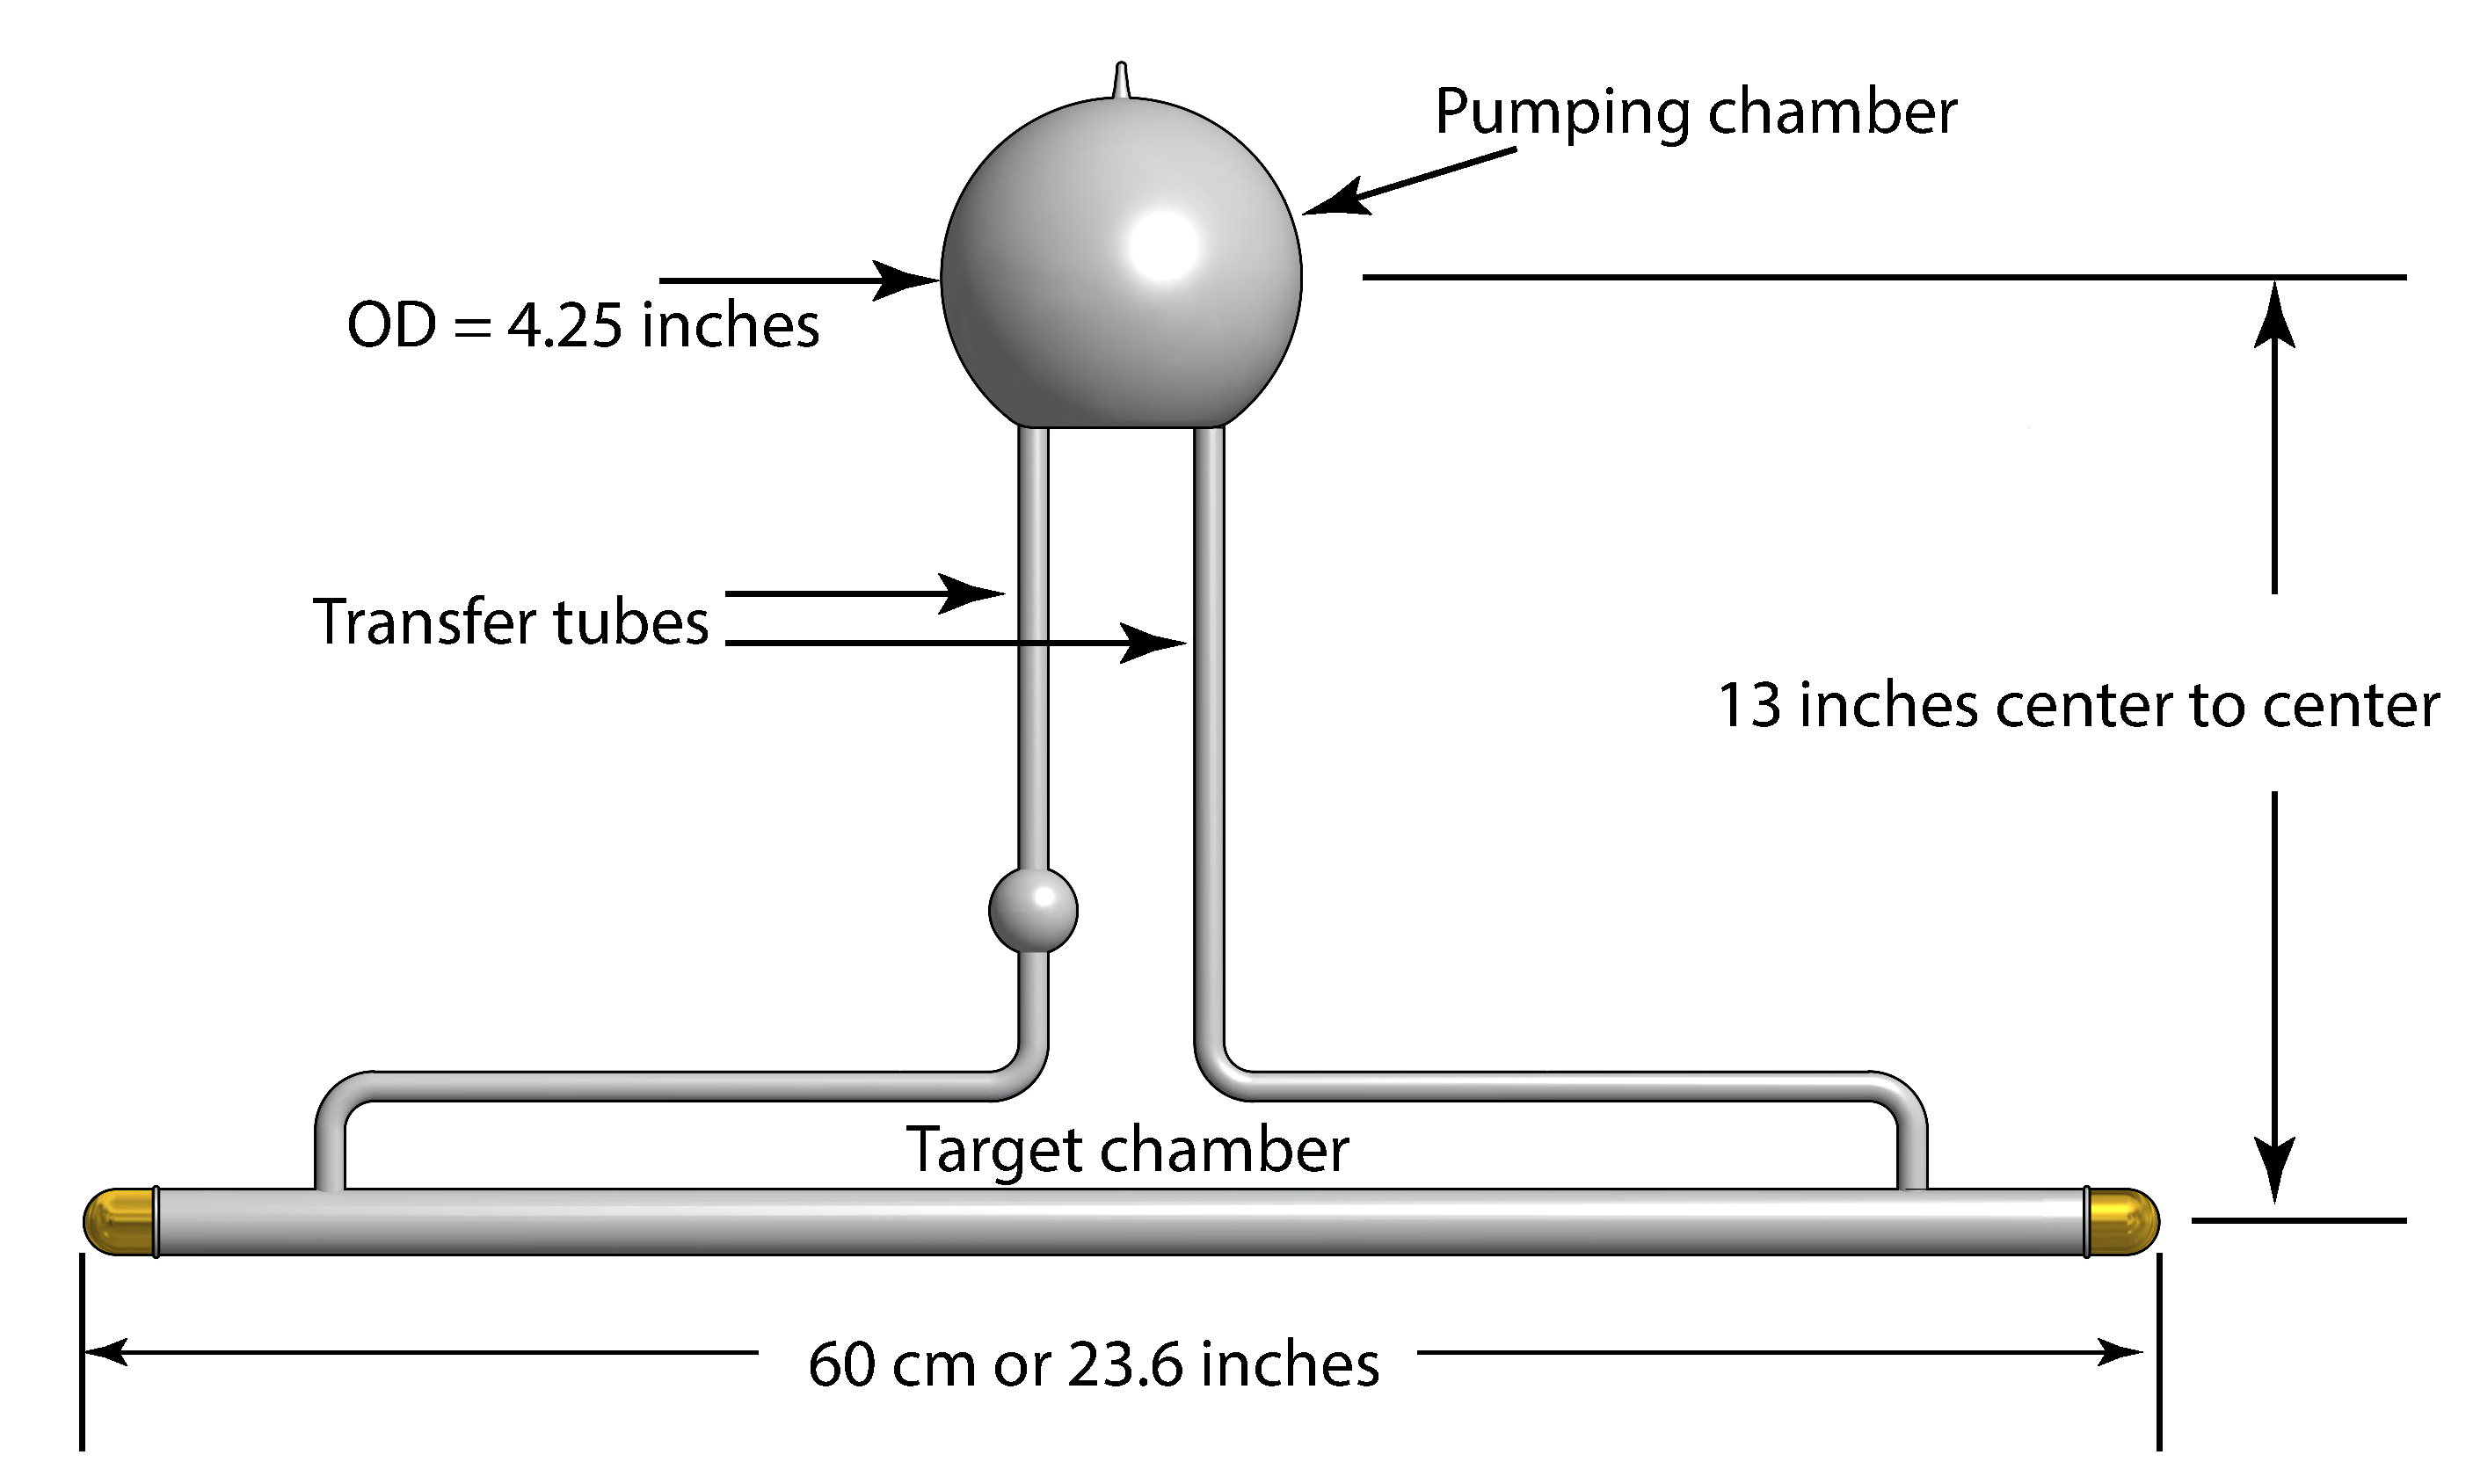
\includegraphics{gen_cell_design_draft_v2.pdf}}
	\caption{{Design of next-generation target for upcoming SBS $G_E^n$ experiments.}}
	\label{Next_Gen_Design}
\end{figure}

\section{Overall Design of Next-Generation Polarized $^3$He Targets}

The target-cell design illustrated in Fig.~\ref{Next_Gen_Design} incorporates multiple features that distinguish it from earlier polarized $^3$He targets based on spin-exchange optical pumping. The basic geometry is what we refer to as a ``convection-style" cell, in which the pumping and target chambers are connected
by two transfer tubes, one of which is heated, resulting in controllable convective flow between the target's two principle chambers. The development of convection-style cells was an important part of the thesis work of Peter Dolph, and is well documented in Ref.~\cite{PhysRevC.84.065201}. Subsequent to the work described in~\cite{PhysRevC.84.065201}, our group constructed and tested two convection-style prototype target cells. 

Another distinguishing feature of the design shown in Fig.~\ref{Next_Gen_Design} is that it is significantly larger than previous target cells, containing 6 STP liters of $^3$He, and has a target chamber that is 60 cm in length, 50\% longer than any target cells previously operated at JLab.  The confidence that this target will achieve polarization $>$ 60\% in ${\rm 60\,\mu A}$ of beam came as a direct result of the work described in Chapter 4, and published in Ref.~\cite{PhysRevC.91.055205}. While much of the data presented in Ref.~\cite{PhysRevC.91.055205} were obtained prior to the work described here, most of the analysis was performed as part of this work, including a determination of the coefficient characterizing spin-exchange between potassium and $^3$He.  

Data included in ref.~\cite{PhysRevC.91.055205} that were specifically obtained as part of this thesis work included all of the studies of the cell Antoinette, which contained roughly 3 STP liters of $^3$He. While target-cells containing 3 STP liters of $^3$He were used during the first Hall A $G_E^n$ experiment (E02-013), commercial narrow-band high-power diode-laser arrays, which are critical to achieving high performance, were not yet available during both testing and the experiment itself. Thus, Antoinette was the first target cell tested with narrow-band lasers that contained both 3 STP liters of $^3$He and an alkali-hybrid mixture for optical pumping. As such, Antoinette became a proof of principle for both of the above-mentioned prototype convection-style target cells, as well as the first production Stage-I target cell that is undergoing testing at the time of this writing.

In short, the work presented here provided the basis for designing the high-performance Stage-I and Stage-II target cells that will be used in future JLab experiments. The proof-of-principle began with the cell Antoinette, and continued with the two prototype convection-style target cells (both of which
also contained roughly 3 STP liters of $^3$He). The first actual Stage-I target cell looks very promising in early tests, providing further confidence in the design of the Stage-II target cells that will soon be produced.

\section{Incorporating Metal End Windows}

Prior to the work described here, there was only very limited experience with spin-polarized noble gases in cells containing metal. The reason is that the introduction of any new material  generally causes spin relaxation greatly in excess to that caused by the walls of the glass container. The target-cell design shown in Fig.~\ref{Next_Gen_Design}, however, incorporates metal end windows so that even a fairly intense electron beam will not cause the target cell to rupture, even after multiple weeks of operation. One of the important achievements
of the current work was the development of a technique for producing metal surfaces that induce spin relaxation at an acceptably slow rate. We further have demonstrated a means for making transitions between glass and metal, even when operating at the high pressures used in our polarized $^3$He targets. We describe
next why metal end windows based on the techniques demonstrated here are likely to have an almost negligible effect on the overall performance of our target cells.

The spin relaxation caused by metal end windows in future target cells can be calculated using the equation $\Gamma_{metal} = \rho_{metal} S_{metal}/V_{total}$ (see Chapter 2.4). Furthermore, the relaxivity associated with metal can be extracted by comparing a glass-and-metal test cell (such as GoldRush in Table.~\ref{test_cells}) with an all-glass control cell (such as Pyrah in Table.\ref{test_cells}). The relaxivity for Pyrah can be computed to be 0.0314 cm/hr, and when compared with GoldRush, indicates a relaxivity of 0.123 cm/hr for the metal. Using this relaxivity and the design dimensions for the target end windows, the additional relaxation times would be 1/93.06 hr$^{-1}$ for Stage-I cells and 1/186.12 hr$^{-1}$ for Stage-II cells.

During the 6 GeV era where only 10-15 $\mu$A was used, glass end windows were already running into risk of rupturing after 4-6 weeks of being exposed to the electron beam. If rupturing was solely due to radiation damage, one would expect the glass windows to rupture after roughly a week of being used in an electron beam of 60 $\mu$A, which would be much less than the time required for the experiment to complete. On the other hand, experience at JLab suggests that even very thin metal windows would be able to survive the electron beam. As a an example, aluminum as thin as 2 mils has been routinely used in JLab without failing. The fact that metal end windows will conduct heat better further suggests that they will be more suitable for the planned experiment. While some work remains to determine the optimal configuration for the window itself, the work presented here provides the critical technology that previously prevented us from using metal end windows in our targets.

\section{Summary}

We have confidence that convection style targets with metal end windows will not only give high $^3$He polarization in both the pumping and target chambers, but also survive the high electron beam currents planned for the future experiments. The work done in this thesis has demonstrated that the additional spin-relaxation rate due to surfaces in metal end windows will be negligible for our purposes and has provided techniques for connecting metal end windows to glass. All the tests so far have been performed on test cells with metal tubes. Before a target cell with next-generation design can be produced, tests exploring techniques for making hemispherical metal end caps should be carried out. However, with techniques established so far, we believe the next-generation design will be used to great success in the upcoming experiments planned for the 12 GeV era.
